\chapter{Orchestration BPMN}\label{chap:bpmn}

\section{Outil et principe}
Le processus « Traitement d'une candidature de stage » est modélisé en \textbf{BPMN 2.0} standard
(\code{candidature-stage.bpmn20.xml}, modèle et diagramme BPMN-DI) et exécuté par le moteur \textbf{Flowable},
embarqué dans la plateforme. Flowable est l'« outil équivalent » à Bonita autorisé par le sujet : il exécute le même
standard, ce qui permet de démontrer une orchestration \emph{réellement exécutée} et testée automatiquement. Le fichier
reste importable dans Bonita Studio, Camunda Modeler ou bpmn.io (procédure en section~\ref{sec:bonita}).

Chaque \textbf{tâche de service} est reliée à un délégué Java qui appelle un service SOAP ou REST \emph{par le
réseau}, exactement comme le ferait un connecteur Bonita. Les tâches humaines (décision de l'entreprise, traitement
d'un incident) sont exposées par l'API \code{/api/processus} et l'interface web.

\begin{sidewaysfigure}
\centering
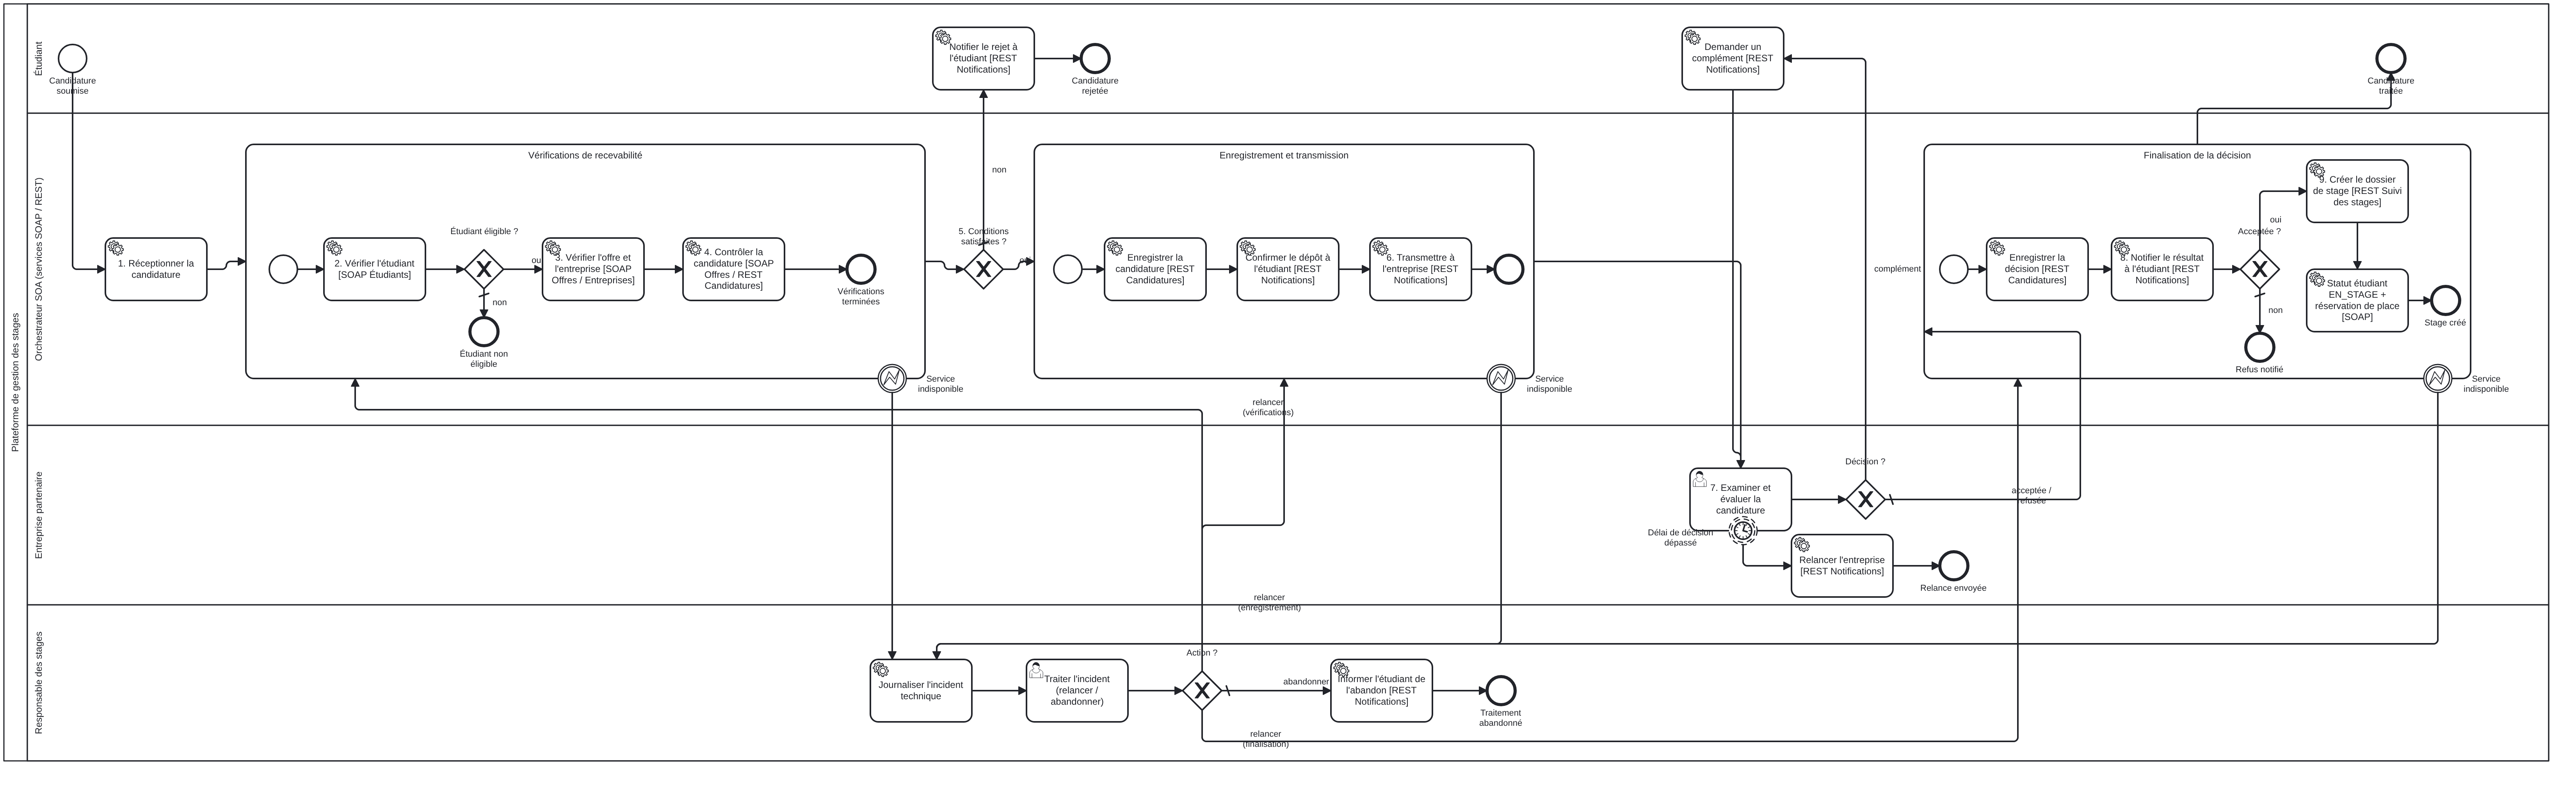
\includegraphics[width=\textheight]{figures/processus-bpmn.png}
\caption{Diagramme BPMN du processus de traitement d'une candidature (rendu bpmn-js du fichier exécuté)}\label{fig:bpmn}
\end{sidewaysfigure}

\section{Structure du processus}
Le pool « Plateforme de gestion des stages » comporte quatre couloirs : \emph{Étudiant}, \emph{Orchestrateur SOA},
\emph{Entreprise partenaire} et \emph{Responsable des stages}. Les étapes de l'orchestrateur sont regroupées en
trois \textbf{sous-processus} qui délimitent les zones de reprise en cas d'erreur.

\begin{table}[htbp]
\centering\small
\caption{Correspondance entre les étapes du sujet et le modèle BPMN}\label{tab:etapes}
\begin{tabularx}{\textwidth}{@{}lYY@{}}
\toprule
\textbf{Étape du sujet} & \textbf{Éléments BPMN} & \textbf{Service appelé} \\
\midrule
1. Réception & Événement de début « Candidature soumise » ; tâche « Réceptionner » (contrôle de forme, initialisation) & API \code{POST /processus/candidatures} \\
2. Vérification de l'étudiant & Tâche « Vérifier l'étudiant » ; passerelle « Étudiant éligible ? » & SOAP Étudiants : \code{verifierEtudiant}, \code{consulterEtudiant} \\
3. Vérification de l'offre & Tâche « Vérifier l'offre et l'entreprise » & SOAP Offres : \code{consulterOffre}, \code{verifierCompatibilite} ; SOAP Entreprises : \code{verifierEntreprise}, \code{consulterEntreprise} \\
4. Contrôle de la candidature & Tâche « Contrôler la candidature » & SOAP Offres : \code{verifierDisponibilite} ; REST : \code{GET /candidatures} (doublon) \\
5. Passerelle de décision & Passerelle exclusive « Conditions satisfaites ? » : rejet notifié \emph{ou} enregistrement & REST : \code{POST /notifications} \emph{ou} \code{POST /candidatures} \\
6. Transmission à l'entreprise & Sous-processus « Enregistrement et transmission » : confirmation à l'étudiant, notification de l'entreprise & REST Notifications \\
7. Décision de l'entreprise & Tâche humaine « Examiner et évaluer la candidature » : prise en charge (statut « en cours d'évaluation »), puis passerelle « Décision ? » (accepter, refuser, demander un complément) & API \code{…/prise-en-charge} puis \code{…/decision} ; REST \code{PATCH /candidatures/\{id\}/statut} \\
8. Notification du résultat & Tâche « Notifier le résultat » (gabarit ACCEPTATION ou REFUS) & REST Notifications \\
9. Mise à jour du suivi & Passerelle « Acceptée ? » ; « Créer le dossier de stage » ; « Statut EN\_STAGE + réservation de place » & REST : \code{POST /stages} ; SOAP : \code{changerStatutEtudiant}, \code{reserverPlace} \\
\bottomrule
\end{tabularx}
\end{table}

\section{Passerelles et conditions}
\begin{table}[htbp]
\centering\small
\caption{Passerelles exclusives et expressions de condition}
\begin{tabularx}{\textwidth}{@{}lYl@{}}
\toprule
\textbf{Passerelle} & \textbf{Branches (condition JUEL)} & \textbf{Défaut} \\
\midrule
Étudiant éligible ? & oui : \code{\$\{etudiantEligible\}} & fin « Étudiant non éligible » \\
Conditions satisfaites ? & oui : \code{\$\{recevable\}} → enregistrement & notification du rejet \\
Décision ? & complément : \code{\$\{decision == 'COMPLEMENT'\}} → notification puis retour à l'évaluation & finalisation \\
Acceptée ? & oui : \code{\$\{decision == 'ACCEPTEE'\}} → création du stage & fin « Refus notifié » \\
Action ? (incident) & relancer : \code{\$\{actionIncident == 'RELANCER' \&\& etapeCourante == '…'\}} (une branche par sous-processus) & abandon notifié \\
\bottomrule
\end{tabularx}
\end{table}

La variable \code{recevable} n'est vraie que si l'étudiant est actif, l'offre active, l'entreprise référencée, la
filière et le niveau compatibles, la date limite non dépassée, une place disponible, aucune candidature non annulée
n'existe pour le même couple étudiant/offre, et l'étudiant a moins de 5 candidatures en cours. Tous les motifs de refus sont accumulés dans \code{motifRejet} et repris
dans la notification adressée à l'étudiant.

\section{Gestion des erreurs et des indisponibilités}\label{sec:erreurs}
La gestion des erreurs est organisée en quatre niveaux.

\paragraph{1. Reprise automatique.} Tout appel inter-services passe par \code{Resilience.avecReprise} :
3 tentatives avec un délai exponentiel (400~ms, 800~ms), délais de connexion et de réponse bornés à 5~s.
Seules les erreurs \emph{techniques} sont rejouées (connexion impossible, délai dépassé, HTTP 5xx) ; une erreur
\emph{fonctionnelle} (HTTP 4xx, SOAP Fault métier) est propagée immédiatement.

\paragraph{2. Erreur BPMN et événement de bordure.} Si le service reste indisponible, le délégué lève
\code{BpmnError("ERREUR\_TECHNIQUE")} après avoir renseigné \code{serviceEnErreur}, \code{messageErreur} et
\code{activiteEnErreur}. Chacun des trois sous-processus porte un \textbf{événement d'erreur de bordure} « Service
indisponible » qui interrompt le sous-processus et dirige le flux vers « Journaliser l'incident ».

\paragraph{3. Traitement humain de l'incident.} La tâche « Traiter l'incident » est attribuée au responsable des
stages, qui choisit de \textbf{relancer} l'étape — le flux revient au début du sous-processus en erreur, identifié par
la variable \code{etapeCourante} positionnée par un écouteur d'exécution — ou d'\textbf{abandonner}, auquel cas
l'étudiant est informé et l'instance se termine par l'événement « Traitement abandonné ».

\paragraph{4. Notifications non bloquantes.} Une notification non envoyée ne justifie pas de bloquer un étudiant :
après les reprises, l'échec est consigné dans la variable \code{incidents} et le processus continue.

\begin{lstlisting}[language=Java, caption={Conversion d'une indisponibilité en erreur BPMN (\code{AbstractServiceDelegate})}]
@Override
public final void execute(DelegateExecution execution) {
    try {
        executer(execution);
    } catch (ServiceIndisponibleException e) {
        String msg = "Service « " + e.getService() + " » indisponible : " + e.getMessage();
        execution.setVariable("serviceEnErreur", e.getService());
        execution.setVariable("messageErreur", msg);
        execution.setVariable("activiteEnErreur", execution.getCurrentActivityId());
        throw new BpmnError(ERREUR_TECHNIQUE, msg);   // intercepté par l'événement de bordure
    }
}
\end{lstlisting}

\paragraph{Idempotence des reprises.} Relancer un sous-processus ne doit pas dupliquer les effets déjà produits :
l'enregistrement de la candidature est ignoré si \code{candidatureId} est déjà connu, la création du stage récupère le
stage existant en cas de réponse \code{409}, et la réservation de place est mémorisée par \code{placeReservee}.

\paragraph{Démonstration.} Le simulateur de pannes (\code{POST /api/admin/pannes} ou écran « Supervision ») rend
n'importe lequel des six services indisponible (HTTP~503) ; les scénarios PT-04 à PT-06 du chapitre~\ref{chap:tests}
vérifient automatiquement ces comportements.

\section{Autres mécanismes}
\begin{description}[style=nextline]
  \item[Minuteur de relance] Un événement minuteur de bordure \textbf{non interrompant} est attaché à « Évaluer la
        candidature ». Passé le délai (\code{P3D} par défaut, paramétrable), l'entreprise est relancée par une
        notification \code{RELANCE\_DECISION} sans que la tâche d'évaluation soit annulée.
  \item[Prise en charge] La candidature reste \code{DEPOSEE} — donc annulable par l'étudiant — tant que l'entreprise
        n'a pas ouvert le dossier. Le bouton « Examiner » attribue la tâche à l'entreprise (\emph{claim}) et fait passer la
        candidature \code{EN\_COURS\_EVALUATION} ; une décision rendue directement déclenche cette prise en charge.
  \item[Demande de complément] La branche « complément » de la passerelle « Décision ? » notifie l'étudiant puis revient
        à la tâche d'évaluation ; l'étudiant complète son dossier par \code{PATCH /candidatures/\{id\}}.
  \item[Annulation] Lorsqu'un étudiant annule sa candidature, le service Candidatures publie un événement
        « candidature annulée » ; l'orchestrateur, abonné, interrompt l'instance correspondante (statut \code{INTERROMPU}).
  \item[Cohérence] Une décision ne peut pas contourner le processus : un \code{PATCH} manuel vers \code{ACCEPTEE} ou
        \code{REFUSEE} sur une candidature orchestrée est refusé (\code{409 DECISION\_VIA\_PROCESSUS}).
  \item[Traçabilité] L'historique du moteur est exposé par \code{GET /processus/instances/\{id\}} : activités
        traversées avec horodatage et durée, activités actives, variables, raison d'arrêt. L'interface superpose ces
        informations au diagramme (figure~\ref{fig:ui-instance}).
\end{description}

\section{Reproduction dans Bonita Studio}\label{sec:bonita}
Le guide \code{docs/bonita/GUIDE\_BONITA.md} détaille la reproduction du processus dans Bonita :
\begin{enumerate}
  \item importer \code{docs/bonita/traitement-candidature-bonita.bpmn} (\emph{Fichier › Importer › BPMN 2.0}), variante
        préparée pour Bonita : flux à plat (Bonita ne gère pas les sous-processus embarqués), un événement d'erreur de
        bordure sur chaque tâche critique, aucune extension propriétaire, noms de tâches courts adaptés à la taille fixe
        des tâches de Bonita. L'import a été vérifié dans Bonita Studio ;
  \item déclarer les variables du processus (tableau du guide) ;
  \item associer à chaque tâche de service un connecteur \emph{Web Service SOAP} ou \emph{REST} (même opérations
        qu'au tableau~\ref{tab:etapes}, compte \code{systeme}) ;
  \item configurer \emph{Lever un événement d'erreur} en cas d'échec des connecteurs critiques, et \emph{Ignorer
        l'erreur} pour les notifications ;
  \item définir les acteurs \emph{entreprise} et \emph{responsable} ainsi que le minuteur non interrompant.
\end{enumerate}
